
%\documentclass[manuscript]{acmart}
%\documentclass[acmsmall]{acmart}
%\settopmatter{printacmref=false}


\documentclass[
  a4paper,
  12pt,
  DIV=12,        % höherer Wert = schmalere Ränder, weniger Whitespacmi
  parskip=half,  % Absätze mit halbem Abstand statt Einzug
  headings=small % kleinere Überschriften, weniger vertikaler Abstand
]{scrartcl}

%\documentclass[a4paper,11pt]{scrartcl}
%\documentclass[a4paper,11pt]{report}
%\documentclass[a4paper,12pt]{book}
\usepackage[utf8]{inputenc}
\usepackage[german]{babel}
\usepackage[T1]{fontenc}
\usepackage{lmodern}
\usepackage[inkscapelatex=false]{svg}
% Texte im SVG von Inkscape setzen lassen, nicht durch die Dokumentschrift ersetzen
\svgsetup{inkscapelatex=false}
\usepackage{amsmath}
\usepackage{caption}
\usepackage{gensymb}
\usepackage{microtype}
\usepackage{longtable}
\usepackage{tabularx}   % Spalten, die die restliche Zeilenbreite auffüllen (X-Spalte)
\usepackage{booktabs}   % \toprule \midrule \bottomrule (in mobrob_table.tex verwendet)
\usepackage{wrapfig}    % Textumfluss um Abbildungen
\usepackage{array}
\usepackage{calc}

\usepackage[citecolor=black, colorlinks=true, linkcolor=black, urlcolor=blue]{hyperref}


%\usepackage{geometry}
\usepackage{siunitx}
%\geometry{margin=2.5cm}


\usepackage{amsthm}
\usepackage{mdframed}
\usepackage{enumitem}

\newmdtheoremenv{theorem}{Theorem}

\theoremstyle{definition}
\newmdtheoremenv{derivation}{Derivation}

\providecommand{\tightlist}{%
  \setlength{\itemsep}{0pt}\setlength{\parskip}{0pt}}

%\mdfdefinestyle{leftline}{
%    topline=false, bottomline=false, rightline=false,
%    linewidth=2pt, linecolor=gray
%}
\theoremstyle{definition}
\newmdtheoremenv[style=leftline]{myalgorithm}{Algorithm}




%\usepackage{fancyvrb}







\let\Bbbk\relax
\usepackage{amssymb}


\usepackage{yfonts}

\usepackage{kvmap}

\usepackage[
    backend=biber,
    style=alphabetic,
    sortlocale=de_DE,
    natbib=true,
    %url=false,
    doi=true,
    %eprint=false
]{biblatex}
% \addbibresource{Literaturrecherche-Stefan-Etringer/algo-references.bib}

%\usepackage[
%    backend=biber,
%    style=alphabetic,
%    sortlocale=de_DE,
%    natbib=true,
%    %url=false,
%    doi=true,
%    %eprint=false
%]{biblatex}
%\addbibresource{Literaturrecherche-Dennis/mobrob_references.bib}

\usepackage[autostyle=true,german=quotes]{csquotes}
\usepackage{trfsigns} %fourier transform arrow
\usepackage{mathrsfs} %fourier F
\usepackage{commath}

\usepackage{pgfplots}
\pgfplotsset{compat=1.18}

\usepackage{xcolor}
\usepackage{listings}
\usepackage[european]{circuitikz}
\ctikzset{tripoles/european not symbol=ieee circle}

%\usepackage[shading]{moeptikz}
%\moeptikzset{shading=true}

%\usepackage{german,longtable}

\usepackage{xcolor}
\usepackage{color}
\usepackage{url}

\usepackage{xfrac}

\usepackage{listings}
\usepackage{verbatimbox}

\usepackage{algorithm}
\usepackage{algpseudocode}

\usepackage{multirow}
\usepackage{float}
\usepackage{pdflscape}   % einzelne Querformatseiten (im PDF gedreht)

%%%% TIKZ

\usepackage{tikz}

\usepackage{pgfplots}
\usetikzlibrary{calc,
trees,positioning,arrows,
chains,shapes.geometric,
decorations.pathreplacing,
decorations.pathmorphing,shapes,
matrix,shapes.symbols,
plotmarks}
%\tikzexternalize[prefix=figures/]

%\tikzset{%
%  block/.style    = {draw, thick, rectangle, minimum height = 3em,
%    minimum width = 3em},
%  sum/.style      = {draw, circle, node distance = 2cm}, % Adder
%  input/.style    = {coordinate}, % Input
%  output/.style   = {coordinate} % Output
%}
% Defining string as labels of certain blocks.
%\newcommand{\suma}{\Large$+$}
%\newcommand{\multa}{\Large$\times$}
%\newcommand{\inte}{$\displaystyle \int$}
%\newcommand{\derv}{\huge$\frac{d}{dt}$}

\usetikzlibrary{arrows,automata,positioning}
%\usepackage{automata}


%%% END TIKZ

\usepackage[section]{placeins}

\usepackage{textcomp}


\usepackage{listings}
\usepackage{verbatimbox}

\usepackage{bold-extra}

\usepackage{framed}

%\usepackage{fancyhdr}
%\pagestyle{fancy}
%\lhead{\leftmark}
%\chead{}
%\rhead{}
%\lfoot{}
%\cfoot{\thepage}
%\rfoot{}
%\renewcommand{\headrulewidth}{0.2pt}
%\renewcommand{\footrulewidth}{0.2pt}



\newcommand{\Z}{\mathbb{Z}}
\newcommand{\R}{\mathbb{R}}
\newcommand{\C}{\mathbb{C}}
\newcommand{\N}{\mathbb{N}}
\newcommand{\SqrtNy}{$\sqrt{\textsc{Ny}}$}
\newcommand{\conj}{\overline}
\newcommand{\Kset}{\textswab{K}}
\newcommand{\Qset}{\textswab{Q}}
\newcommand{\ceil}[1]{\left\lceil #1 \right\rceil}
\newcommand{\floor}[1]{\left\lfloor #1 \right\rfloor}
\newcommand{\sorted}[1]{\textsc{sort}\left\lbrace #1 \right\rbrace}
\newcommand{\SNRgain}{a_{SNR}}
\newcommand{\EQgain}{a_{EQ}}
\newcommand{\SIRgain}{a_{SIR}}
\newcommand{\SNIRgain}{a_{SINR}}
\newcommand{\SNR}{\textsc{SNR}}
\newcommand{\CIRgain}{a_{CIR}}
\newcommand{\CINRgain}{a_{CINR}}
\newcommand{\CNR}{\textsc{CNR}}
\newcommand{\CINR}{\textsc{CINR}}
\newcommand{\HPAModel}{ Hughes 1177H TWTA }
\newcommand{\bigO}{\mathcal{O}}
\newcommand{\CopWinCompl}{2.375377}
\newcommand{\IBO}{\textsc{IBO}}
\newcommand{\OBO}{\textsc{OBO}}
\newcommand{\spacepage}{\newpage\null\thispagestyle{empty}\newpage}
\newcommand{\satcom}{ SatCom }
\newcommand{\db}{~\text{dB}}


\definecolor{mGreen}{rgb}{0,0.6,0}
\definecolor{mGray}{rgb}{0.5,0.5,0.5}
\definecolor{mPurple}{rgb}{0.58,0,0.82}
\definecolor{backgroundColour}{rgb}{0.95,0.95,0.92}

\lstdefinestyle{CStyle}{
    backgroundcolor=\color{backgroundColour},
    commentstyle=\color{mGreen},
    keywordstyle=\color{magenta},
    numberstyle=\tiny\color{mGray},
    stringstyle=\color{mPurple},
    basicstyle=\footnotesize,
    breakatwhitespace=false,
    breaklines=true,
    captionpos=b,
    keepspaces=true,
    numbers=left,
    numbersep=5pt,
    showspaces=false,
    showstringspaces=false,
    showtabs=false,
    tabsize=2,
    language=C
}

\lstdefinelanguage{VHDL}{
  morekeywords=[1]{library,use,all,entity,is,port,in,out,end,architecture,of,begin,process,if,then,else,elsif,when,others,signal,variable,wait,for,loop},
  morecomment=[l]--,
  morestring=[b]",
  sensitive=true
}

\lstset{
  language=VHDL,
  basicstyle=\ttfamily\small,
  keywordstyle=\color{blue},
  commentstyle=\color{gray},
  stringstyle=\color{red},
  numbers=left,
  numberstyle=\tiny,
  stepnumber=1,
  numbersep=8pt,
  frame=single,
  breaklines=true,
  captionpos=b
}

\lstset{numbers=none}

%\newcounter{example}
%\renewcommand{\theexample}{\thesection.\arabic{example}}


% Default fixed font does not support bold face
\DeclareFixedFont{\ttb}{T1}{txtt}{bx}{n}{12} % for bold
\DeclareFixedFont{\ttm}{T1}{txtt}{m}{n}{12}  % for normal

% Custom colors
\usepackage{color}
\definecolor{deepblue}{rgb}{0,0,0.5}
\definecolor{deepred}{rgb}{0.6,0,0}
\definecolor{deepgreen}{rgb}{0,0.5,0}

\usepackage{listings}

% Python style for highlighting
\newcommand\pythonstyle{\lstset{
language=Python,
basicstyle=\ttm,
morekeywords={self},              % Add keywords here
keywordstyle=\ttb\color{deepblue},
emph={MyClass,__init__},          % Custom highlighting
emphstyle=\ttb\color{deepred},    % Custom highlighting style
stringstyle=\color{deepgreen},
frame=tb,                         % Any extra options here
showstringspaces=false
}}


% Python environment
\lstnewenvironment{python}[1][]
{
\pythonstyle
\lstset{#1}
}
{}

% Python for external files
\newcommand\pythonexternal[2][]{{
\pythonstyle
\lstinputlisting[#1]{#2}}}

% Python for inline
\newcommand\pythoninline[1]{{\pythonstyle\lstinline!#1!}}


% ---------------------------------------------------------------------
% Stil fuer C++-Listings dieser Dokumentation
% ---------------------------------------------------------------------
\lstdefinestyle{cpp}{
  language=C++,
  basicstyle=\ttfamily\footnotesize,
  keywordstyle=\color{deepblue},
  commentstyle=\color{mGreen},
  stringstyle=\color{mPurple},
  numbers=none,
  breaklines=true,
  showstringspaces=false,
  frame=single,
  columns=fullflexible,
  captionpos=b
}



%\nocite{*}


\begin{document}
%\pagenumbering{roman}



\title{Coasterbot}
\subtitle{Softwaredokumentation}
\author{Stefan Etringer}
%\email{gereonsuch@suchdsp.com}
%\affiliation{
%  \institution{Wilhelm Büchner University of Applied Sciences}
%  \department{Computer Engineering}
%  \city{Hof}
%  \country{Germany}
%}



\begin{titlepage}
  \begin{center}
    {\large Wilhelm Büchner University of Applied Sciences} \\[0.3em]

    {\normalsize Projektseminar Master}
\vspace{5em}

    {\LARGE\bfseries Coasterbot} \\[0.5em]

    {\large Softwaredokumentation} \\[1em]

    {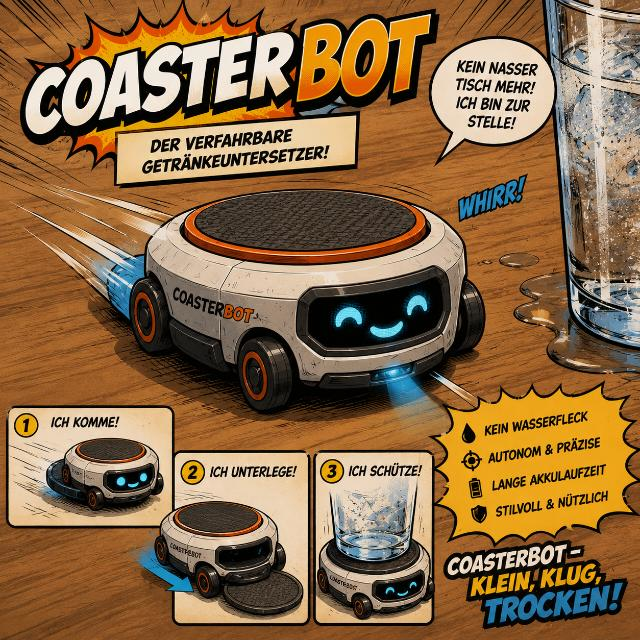
\includegraphics[width=0.38\textwidth]{coasterbot.png}} \\[1em]

\vspace{4em}

    {\normalsize
\begin{tabular}{ll}
Dennis Borutta, B. Eng & dennis.borutta@outlook.com\\
Stefan Etringer, B. Eng & mail@stefan.works\\
Gereon Such, M. Sc. & gereonsuch@gmail.com\\
\end{tabular}
    }
  \end{center}


\end{titlepage}


% einleitung preambel etc.


% Versionshistorie des Dokuments -- eigene Seite direkt nach dem Titelblatt
\section*{Versionshistorie}

\begin{tabularx}{\textwidth}{@{}clp{2.6cm}X@{}}
\toprule
\textbf{Version} & \textbf{Datum} & \textbf{Bearbeiter} & \textbf{Änderungen}\\
\midrule
1 & 08.09.2026 & Etringer & Erstfassung der Softwaredokumentation der Simulationssoftware\\
\bottomrule
\end{tabularx}


\newpage

\tableofcontents

\newpage

% Etwas mehr Toleranz beim Umbruch: viele \texttt{}-Bezeichner sind nicht
% trennbar und wuerden sonst knapp ueber den Satzspiegel ragen.
\setlength{\emergencystretch}{3em}

% =====================================================================
\section{Einleitung}\label{einleitung}
% =====================================================================

\subsection{Zweck des Dokuments}\label{zweck-des-dokuments}

Dieses Dokument beschreibt die \textbf{Software der Simulation des
Coasterbots} sowie deren Funktionen. Dokumentiert wird die
Softwarearchitektur, die einzelnen Softwarekomponenten, ihre
Schnittstellen und ihr Laufzeitverhalten in der Simulationsumgebung.

Grundlage der Dokumentation sind die im Projekt erstellten
Anforderungs- und Testdokumente:

\begin{itemize}
\tightlist
\item
  \textbf{Lastenheft} -- funktionale und nichtfunktionale Anforderungen
  des Auftraggebers (Kennungen \texttt{NAV-*}, \texttt{SAF-*},
  \texttt{MON-*}, \texttt{NFA-*}, \texttt{SIM-*}).
\item
  \textbf{Pflichtenheft} -- geplante technische Umsetzung,
  die geschichtete System- und Softwarearchitektur (Hardwaretreiber,
  Hardwareabstraktion, Systemdienste, Funktionskomponenten,
  Anwendungsebene, Simulationsebene).
\item
  \textbf{Testkonzept} -- Teststrategie und Simulationstestfälle
  (\texttt{ST-SIM-001} bis \texttt{ST-SIM-008}).
\item
  \textbf{Alternativenbeschreibung} -- Auswahl der Navigations- und
  Lokalisierungsalgorithmen (A*, D* Lite, DWA, Sensorfusion).
\end{itemize}

Die Software wurde entsprechend der im Pflichtenheft beschriebenen
Abstraktion umgesetzt: Die eigentliche Systemlogik ist vollständig von
der konkreten Hardware entkoppelt und kommuniziert über
eine Hardwareabstraktionsschicht. Dadurch sind die Funktionen im Quellcode sowohl
in der Simulation (Webots) als auch auf der Zielhardware (Mikrocontroller)
verwendbar.
lauffähig.

\subsection{Gegenstand und Abgrenzung}\label{gegenstand-und-abgrenzung}

Gegenstand dieser Dokumentation ist die Software des
Webots-Controllers \texttt{coasterbot} (C++), die den simulierten
Roboter steuert. Dokumentiert werden:

\begin{itemize}
\tightlist
\item
  die Hardwareabstraktion (\texttt{RobotHAL} / \texttt{WebotsHAL}),
\item
  die Lokalisierung (\texttt{PoseEstimator}),
\item
  das Umgebungsmodell (\texttt{OccupancyGrid}),
\item
  die globale Pfadplanung (\texttt{astarPlan}, A*),
\item
  die dynamische Neuplanung (\texttt{DStarLite}, D* Lite),
\item
  die lokale Kollisionsvermeidung und Bewegungssteuerung
  (\texttt{DwaPlanner}),
\item
  die Sicherheitskomponente (\texttt{SafetyMonitor}),
\item
  die reaktive Verhaltenslogik (\texttt{RobotLogic}),
\item
  die Ablaufsteuerung und Betriebsarten (\texttt{main.cpp}),
\item
  das Simulationsmodell (Webots-Welten und \texttt{Coasterbot}-PROTO).
\end{itemize}

\textbf{Nicht} Bestandteil dieser Dokumentation bzw. der aktuellen
Umsetzung sind:

\begin{itemize}
\tightlist
\item
  das Untersetzerhandling (Aufnahme/Ablage von Getränkeuntersetzern,
  \texttt{CST-*}) einschließlich der Manipulationsplanung (IK + RRT*),
\item
  die missionsbezogene Ablaufsteuerung \texttt{IDLE} $\to$
  \texttt{SEARCH\_COASTER} $\to$ \texttt{PICK\_UP} $\to$ \texttt{TRANSPORT}
  $\to$ \texttt{PLACE} $\to$ \texttt{VERIFY} $\to$ \texttt{DONE},
\item
  eine probabilistische Sensorfusion (EKF/UKF), statt dessen wird ein
  Komplementärfilter verwendet (siehe Abschnitt~\ref{lokalisierung}),
\item
  die Fehlerinjektionstests \texttt{ST-SIM-005} (Sensorausfall) und
  \texttt{ST-SIM-006} (Aktorfehler).
\end{itemize}

Der Umsetzungsstand bezieht sich auf \textbf{Maturity Level~1}
(Prototyp): autonome Navigation, Lokalisierung, sichere Bewegung und
Tischkantenerkennung.

\subsection{Begriffe und Abkürzungen}\label{begriffe-und-abkuerzungen}

\begin{longtable}[]{@{}p{0.22\textwidth}p{0.72\textwidth}@{}}
\toprule
\textbf{Begriff} & \textbf{Bedeutung}\\
\midrule
\endhead
HAL & Hardware Abstraction Layer, Hardwareabstraktionsschicht\\
PROTO & Webots-Modellbeschreibung eines Roboters oder Objekts\\
Pose & Lage des Roboters in der Ebene: $(x, y, \theta)$\\
Belegungskarte & Rasterkarte der Fläche, Zellen frei oder belegt (occupancy grid)\\
A* & heuristischer Graphsuch-Algorithmus für die globale Pfadplanung\\
D* Lite & inkrementeller Neuplaner (Koenig \& Likhachev, 2002)\\
DWA & Dynamic Window Approach, lokale Bewegungsplanung im Geschwindigkeitsraum\\
Carrot-Punkt & vorausliegender Zielpunkt auf dem Pfad (Pure Pursuit)\\
Skid-Steer & Panzerlenkung: Lenkung über Drehzahldifferenz linker/rechter Räder\\
Regelzyklus & ein Simulationsschritt (\texttt{basicTimeStep}), typ.\ \SI{32}{\milli\second}\\
\bottomrule
\end{longtable}

% =====================================================================
\section{Softwarearchitektur}\label{softwarearchitektur}
% =====================================================================

\subsection{Architekturprinzip}\label{architekturprinzip}

Die Software folgt dem im Pflichtenheft (Kapitel \enquote{Softwarekonzept})
beschriebenen \textbf{geschichteten, komponentenbasierten}
Architekturmodell. Jede Schicht hat eine klar abgegrenzte
Verantwortlichkeit und kommuniziert über festgelegte
Schnittstellen mit den benachbarten Schichten. Höhere Schichten kennen
keine Hardware- oder Simulationsdetails.

Die zentrale Abstraktion ist die Hardwareabstraktionsschicht
\texttt{RobotHAL}. Sie ist ein rein abstraktes C++-Interface, das
\emph{weder} Webots \emph{noch} eine konkrete Mikrocontroller-Bibliothek
kennt. Alle Funktionskomponenten (Lokalisierung, Planung, Sicherheit)
sind gegen dieses Interface programmiert. Dadurch werden
die Anforderungen \texttt{NFA-ARC-005}, \texttt{NFA-MAI-001/002} und
\texttt{NFA-SIM-004} erfüllt.

\begin{figure}[H]
\centering
\begin{tikzpicture}[font=\footnotesize,
  layer/.style={draw, rounded corners=1pt, minimum width=11.8cm,
                minimum height=0.9cm, align=center, fill=blue!4},
  sim/.style={draw, rounded corners=1pt, minimum width=11.8cm,
              minimum height=0.9cm, align=center, fill=green!5}]
\node[layer] (app) {\textbf{Anwendungs-/Ablaufsteuerung} \\
  \texttt{main.cpp} -- Betriebsart (\texttt{MODE}), Szenario, Hauptschleife};
\node[layer, below=2mm of app] (fun) {\textbf{Funktionskomponenten} \\
  \texttt{PoseEstimator}, \texttt{astarPlan}, \texttt{DStarLite}, \texttt{DwaPlanner}, \\
  \texttt{SafetyMonitor}, \texttt{RobotLogic}};
\node[layer, below=2mm of fun] (svc) {\textbf{Systemdienste / Modelle} \\
  \texttt{OccupancyGrid} (Umgebungsmodell, Distanzfeld)};
\node[layer, below=2mm of svc] (hal) {\textbf{Hardwareabstraktion} \\
  \texttt{RobotHAL} -- rein abstraktes Interface (Sensoren, Aktoren, Zeit)};
\node[layer, below=2mm of hal] (drv) {\textbf{Hardwaretreiberebene} \\
  \texttt{WebotsHAL} (Webots-C++-API) \quad$|$\quad künftig \texttt{ArduinoHAL}};
\node[sim, below=2mm of drv] (webots) {\textbf{Simulationsebene} \\
  Webots R2025b + \texttt{Coasterbot.proto} (Sensor-/Aktormodelle, Welt)};
\draw[<->] (app) -- (fun);
\draw[<->] (fun) -- (svc);
\draw[<->] (fun.west) to[out=180,in=180] (hal.west);
\draw[<->] (hal) -- (drv);
\draw[<->] (drv) -- (webots);
\end{tikzpicture}
\caption{Schichtenmodell der Simulationssoftware. Die Funktionskomponenten
greifen über \texttt{RobotHAL} auf Sensoren und Aktoren zu.}
\label{fig:schichten}
\end{figure}

\subsection{Abbildung auf die Pflichtenheft-Architektur}\label{abbildung-pflichtenheft}

Tabelle~\ref{tab:mapping-arch} ordnet die im Pflichtenheft definierten
Architekturebenen und Funktionskomponenten den konkreten Quelldateien
des Simulations-Controllers zu.

\begin{longtable}[]{@{}
  >{\raggedright\arraybackslash}p{0.30\textwidth}
  >{\raggedright\arraybackslash}p{0.38\textwidth}
  >{\raggedright\arraybackslash}p{0.22\textwidth}@{}}
\caption{Zuordnung Pflichtenheft-Architektur $\rightarrow$ Umsetzung.}
\label{tab:mapping-arch}\\
\toprule
\textbf{Pflichtenheft} & \textbf{Umsetzung (Datei / Klasse)} & \textbf{Anforderung}\\
\midrule
\endfirsthead
\toprule
\textbf{Pflichtenheft} & \textbf{Umsetzung (Datei / Klasse)} & \textbf{Anforderung}\\
\midrule
\endhead
\bottomrule
\endfoot
Hardware\-treiber\-ebene & \texttt{webots\_hal.cpp} (Geräte-Handles) & --\\
Hardware\-abstraktions\-ebene & \texttt{robot\_hal.h} (\texttt{RobotHAL}), \texttt{webots\_hal} (\texttt{WebotsHAL}) & NFA-ARC-005\\
Systemdienste / Umgebungs\-modell & \texttt{occupancy\_grid} (\texttt{OccupancyGrid}) & SIM-004\\
Navigations\-komponente & \texttt{astar} (A*), \texttt{dstar\_lite} (D* Lite) & NAV-005/008/009\\
Lokalisierungs\-komponente & \texttt{pose\_estimator} (\texttt{PoseEstimator}) & NAV-006, NAV-007\\
Bewegungs\-steuerung & \texttt{dwa\_planner} (\texttt{DwaPlanner::driveVW}), \texttt{robot\_hal.h} & HW-ACT-002/003, SAF-004\\
Sicherheits\-komponente / Sicherheits\-logik & \texttt{safety\_monitor} (\texttt{SafetyMonitor}) & NAV-003/004, SAF-001..005\\
Systemüberwachung & Konsolenprotokoll je Betriebsart in \texttt{main.cpp} & MON-001..005\\
Anwendungsebene & \texttt{main.cpp} (\texttt{MODE}, Szenarien, Hauptschleifen) & --\\
Simulationsebene & \texttt{worlds/*.wbt}, \texttt{Coasterbot.proto} & NFA-SIM-001..005\\
Reaktive Verhaltenslogik (Bring-up) & \texttt{robot\_logic} (\texttt{RobotLogic}) & NAV-001/002, SAF-003\\
\end{longtable}

\subsection{Datenfluss im kombinierten Betrieb}\label{datenfluss}

Abbildung~\ref{fig:datenfluss} zeigt den Datenfluss der Betriebsart
\texttt{MODE\_SIM\_TEST}, in der alle wesentlichen Komponenten
zusammenwirken (Grundlage der Testfälle \texttt{ST-SIM-001} bis
\texttt{ST-SIM-004}).

\begin{figure}[H]
\centering
\resizebox{\textwidth}{!}{%
\begin{tikzpicture}[font=\footnotesize, >=latex, x=1cm, y=1cm,
  box/.style={draw, rounded corners=1pt, align=center, minimum height=9mm,
              inner sep=3pt, fill=blue!4},
  sens/.style={draw, rounded corners=1pt, align=center, minimum height=9mm,
               inner sep=3pt, fill=black!4},
  safe/.style={draw, rounded corners=1pt, align=center, minimum height=9mm,
               inner sep=3pt, fill=red!6}]

% obere Zeile: Lokalisierung
\node[sens] (enc)  at (0,0)   {Encoder\\+ Gyro};
\node[box]  (pose) at (6.6,0) {\texttt{PoseEstimator} $(x,y,\theta)$};

% Mittelzeile: Planungs-Pipeline
\node[sens] (us)    at (0,-1.8)    {Ultraschall};
\node[box]  (grid)  at (2.7,-1.8)  {\texttt{OccupancyGrid}\\+ Distanzfeld};
\node[box]  (dstar) at (6.2,-1.8)  {\texttt{DStarLite}};
\node[box]  (smooth)at (9.3,-1.8)  {\texttt{smoothPath}\\\texttt{centerPath}};
\node[box]  (dwa)   at (12.6,-1.8) {\texttt{DwaPlanner}\\$(v,\omega)$};

% untere Zeile: Sicherheit + Aktorik
\node[sens] (edge)   at (0,-3.6)   {Kantensensoren};
\node[safe] (safety) at (2.9,-3.6) {\texttt{SafetyMonitor}};
\node[box]  (mot)    at (12.6,-3.6){\texttt{RobotHAL} $\rightarrow$ Aktorik};

\draw[->] (enc)   -- (pose);
\draw[->] (us)    -- (grid);
\draw[->] (grid)  -- (dstar);
\draw[->] (dstar) -- (smooth);
\draw[->] (smooth)-- (dwa);
\draw[->] (pose.south) to[out=-90,in=90] (dstar.north);
\draw[->] (pose.north) to[out=90,in=90] (dwa.north);
\draw[->] (dwa)   -- (mot);
\draw[->] (edge)  -- (safety);
\draw[->] (safety.south) |- node[pos=0.25,below]{Vorrang} (mot.west);
\end{tikzpicture}}
\caption{Datenfluss in \texttt{MODE\_SIM\_TEST}. Die Sicherheitskomponente
wird in jedem Regelzyklus \emph{vor} der Navigation ausgewertet und
übernimmt bei einem Kantenereignis sofort die Aktorik.}
\label{fig:datenfluss}
\end{figure}

Ablauf eines Regelzyklus:

\begin{enumerate}
\tightlist
\item
  \texttt{hal.step()} -- Simulationsschritt, neue Sensorwerte.
\item
  \texttt{pose.update()} -- Pose aus Radwinkeln und Gyro fortschreiben.
\item
  \texttt{safety.update()} -- Kantensensoren prüfen; hält die
  Sicherheitskomponente die Aktorik, endet der Zyklus hier.
\item
  Kartenpflege -- ein per Ultraschall erkanntes, unkartiertes Hindernis
  bzw.\ eine erkannte Kante wird in die Belegungskarte eingetragen und
  \texttt{DStarLite} benachrichtigt.
\item
  \texttt{planner.setStart()} / \texttt{computeShortestPath()} -- Pfad
  inkrementell aktualisieren.
\item
  \texttt{smoothPath()} + \texttt{centerPath()} -- Pfad glätten und in
  Korridormitte schieben.
\item
  \texttt{dwa.update()} -- kollisionsfreies Geschwindigkeitspaar wählen
  und als Radgeschwindigkeiten ausgeben.
\end{enumerate}

% =====================================================================
\section{Laufzeitumgebung und Projektstruktur}\label{laufzeitumgebung}
% =====================================================================

\subsection{Werkzeuge}\label{werkzeuge}

\begin{longtable}[]{@{}p{0.28\textwidth}p{0.66\textwidth}@{}}
\toprule
\textbf{Element} & \textbf{Beschreibung}\\
\midrule
\endhead
Simulator & Webots R2025b (Nightly-Build, Commit \texttt{033dbaea\ldots})\\
Sprache & C++ (objektorientiert, eine Klasse je Komponente)\\
Build & Webots-\texttt{Makefile.include}, je Controller ein \texttt{Makefile}\\
Robotermodell & \texttt{protos/coasterbot/Coasterbot.proto} (aus CAD abgeleitet)\\
Controller & \texttt{controllers/coasterbot/} (dieser Quellcode)\\
\bottomrule
\end{longtable}

Übersetzen und Ausführen:

\begin{lstlisting}[style=cpp, language=bash]
export WEBOTS_HOME=~/Documents/webots/webots

# nur den Controller bauen
cd controllers/coasterbot && make

# eine Welt starten (GUI)
$WEBOTS_HOME/webots worlds/coasterbot-simtest.wbt

# kopflos / reproduzierbar
$WEBOTS_HOME/webots --mode=fast --no-rendering --stdout --stderr \
    worlds/coasterbot-simtest.wbt
\end{lstlisting}

\subsection{Quelldateien}\label{quelldateien}

\begin{longtable}[]{@{}
  >{\raggedright\arraybackslash}p{0.30\textwidth}
  >{\raggedright\arraybackslash}p{0.62\textwidth}@{}}
\caption{Dateien des Controllers \texttt{coasterbot}.}\label{tab:dateien}\\
\toprule
\textbf{Datei} & \textbf{Inhalt}\\
\midrule
\endfirsthead
\toprule
\textbf{Datei} & \textbf{Inhalt}\\
\midrule
\endhead
\bottomrule
\endfoot
\texttt{robot\_hal.h} & abstraktes Interface \texttt{RobotHAL}, \texttt{enum WheelId}\\
\texttt{webots\_hal.\{h,cpp\}} & \texttt{WebotsHAL : RobotHAL} -- einzige Webots-abhängige Datei\\
\texttt{pose\_estimator.\{h,cpp\}} & \texttt{PoseEstimator} -- Odometrie + Gyro-Fusion\\
\texttt{occupancy\_grid.\{h,cpp\}} & \texttt{OccupancyGrid} -- Rasterkarte, Distanzfeld\\
\texttt{astar.\{h,cpp\}} & \texttt{astarPlan}, \texttt{smoothPath}, \texttt{centerPath}\\
\texttt{dstar\_lite.\{h,cpp\}} & \texttt{DStarLite} -- inkrementeller Neuplaner\\
\texttt{dwa\_planner.\{h,cpp\}} & \texttt{DwaPlanner} -- lokale Planung, Bewegungssteuerung\\
\texttt{safety\_monitor.\{h,cpp\}} & \texttt{SafetyMonitor} -- Sicherheitskomponente\\
\texttt{robot\_logic.\{h,cpp\}} & \texttt{RobotLogic} -- reaktiver Zustandsautomat\\
\texttt{main.cpp} & Betriebsarten, Szenarien, Hauptschleifen\\
\texttt{Makefile} & Liste der zu übersetzenden Quelldateien\\
\bottomrule
\end{longtable}

% =====================================================================
\section{Hardwareabstraktion}\label{hardwareabstraktion}
% =====================================================================

\subsection{Interface \texttt{RobotHAL}}\label{robothal}

\texttt{RobotHAL} (Datei \texttt{robot\_hal.h}) ist eine rein abstrakte
Klasse. Sie beschreibt ausschließlich, \emph{welche} Fähigkeiten der
Roboter besitzt -- nicht, wie sie technisch realisiert werden. Sie
erfüllt \texttt{NFA-ARC-004} (eindeutig definierte Schnittstellen) und
\texttt{NFA-ARC-005} (Hardwareabstraktion).

\begin{longtable}[]{@{}p{0.40\textwidth}p{0.54\textwidth}@{}}
\caption{Methoden von \texttt{RobotHAL}.}\label{tab:hal}\\
\toprule
\textbf{Methode} & \textbf{Bedeutung / Einheit}\\
\midrule
\endfirsthead
\toprule
\textbf{Methode} & \textbf{Bedeutung / Einheit}\\
\midrule
\endhead
\bottomrule
\endfoot
\texttt{bool step()} & ein Regelzyklus; \texttt{false} = Simulation beendet\\
\texttt{void setLeftSpeed(float)} & Sollgeschwindigkeit linke Seite [rad/s], positiv = vorwärts\\
\texttt{void setRightSpeed(float)} & Sollgeschwindigkeit rechte Seite [rad/s]\\
\texttt{float getUltrasonicDistance()} & Abstand nach vorn [m], kleiner = näher\\
\texttt{float getEdgeFrontLeft()} \ldots & vier Kantensensoren; großer Wert = \enquote{kein Boden}\\
\texttt{float getYaw()} & Gierwinkel um die Hochachse [rad]\\
\texttt{float getGyroZ()} & Giergeschwindigkeit um die Hochachse [rad/s]\\
\texttt{float getWheelAngle(WheelId)} & akkumulierter Radwinkel [rad], positiv = vorwärts\\
\texttt{float getTime()} & Laufzeit seit Programmstart [s]\\
\bottomrule
\end{longtable}

\paragraph{Konventionen.}
\begin{itemize}
\tightlist
\item
  \textbf{Vorzeichen:} \texttt{setLeftSpeed}/\texttt{setRightSpeed}
  positiv $\Rightarrow$ Vorwärtsfahrt. Lenkung über die Drehzahl\-differenz
  (Skid-Steer).
\item
  \textbf{Radpaarung:} Die beiden Räder einer Seite sind mechanisch
  gekoppelt und laufen stets gemeinsam (wie beim realen Coasterbot: zwei
  Getriebemotoren je Seite, gemeinsam angesteuert). Es gibt daher
  \emph{keinen} Einzelrad-Befehl. \texttt{enum WheelId} dient nur dem
  Auslesen der vier Encoder.
\item
  \textbf{Kantensensoren:} Rohwert $\approx 0$ auf einer Fläche,
  $\approx 1000$ über einer Kante; Schwelle \num{500}.
\end{itemize}

\subsection{Implementierung \texttt{WebotsHAL}}\label{webotshal}

\texttt{WebotsHAL} (Datei \texttt{webots\_hal.cpp}) ist die einzige
Datei, die die Webots-C++-API einbindet. Bei einer Portierung auf die
Zielhardware wird nur diese Datei durch eine \texttt{ArduinoHAL} mit
identischer Signatur ersetzt; die übrigen Komponenten bleiben
unverändert.

Aufgaben:

\begin{itemize}
\tightlist
\item
  Beschaffung der Geräte-Handles über die im PROTO vergebenen Namen: die
  gekoppelten Motoren \texttt{wheel\_left::front} und
  \texttt{wheel\_right::front}, die vier Encoder
  \texttt{wheel\_*\_sensor}, der Ultraschall \texttt{ultrasonic}, die vier
  Kantensensoren \texttt{edge\_*}, sowie \texttt{inertial\_unit} und
  \texttt{gyro}. Die Namensstrings sind der Vertrag zwischen PROTO und
  Software.
\item
  Betrieb der Antriebsmotoren im Geschwindigkeitsmodus
  (\texttt{setPosition(\ensuremath{\infty})}).
\item
  \textbf{Vorzeichenkorrektur:} Das Radmodell des PROTO rollt den
  Roboter bei positiver Motordrehzahl nach $+Z$ (Rückseite). Da die
  HAL-Konvention \enquote{positiv = vorwärts} lautet und die Vorderseite
  bei $-Z$ liegt, negiert \texttt{WebotsHAL} die Motor- und
  Encoder-Werte.
\item
  \textbf{Gierrate:} Das Y-up-PROTO wird in der Z-up-Welt mit
  \texttt{rotation 1 0 0 1.5708} aufgestellt. Die Welt-Hochachse fällt
  daher mit der lokalen $+Y$-Achse des Gyros zusammen; \texttt{getGyroZ()}
  liefert die $Y$-Komponente des Gyrovektors.
\end{itemize}

Die coupled motors von Webots setzen einen Befehl an
\texttt{wheel\_left::front} automatisch auch auf
\texttt{wheel\_left::rear} um (Faktor \texttt{multiplier} $= 1$), sodass
die Software je Seite nur ein Handle benötigt.

% =====================================================================
\section{Lokalisierungskomponente}\label{lokalisierung}
% =====================================================================

Die Lokalisierung (\texttt{PoseEstimator}, Dateien
\texttt{pose\_estimator.\{h,cpp\}}) bestimmt fortlaufend die Pose des
Roboters in der Tischebene und erfüllt \texttt{NAV-006}
(Positionsbestimmung) und \texttt{NAV-007} (Orientierungsbestimmung).

\subsection{Prinzip}\label{lokalisierung-prinzip}

Der Coasterbot \emph{misst} seine Position nicht, sondern \textbf{führt
sie durch Koppelnavigation (Dead Reckoning) fort}. Es gibt keine externe
Referenz -- kein GPS, keine Bake, keine kamerabasierte Lokalisierung.
Die Pose entsteht in vier Schritten:

\begin{enumerate}
\tightlist
\item
  \textbf{Bekannte Startpose.} \texttt{main.cpp} setzt den Schätzer über
  \texttt{pose.reset(x,\,y,\,\ensuremath{\theta})} auf die im
  Szenario/in der Welt definierte Startposition. Alles Weitere ist
  relativ zu diesem Punkt.
\item
  \textbf{Radodometrie.} In jedem Regelzyklus werden die vier
  Radencoder (\texttt{wheel\_*\_sensor}) über
  \texttt{RobotHAL::getWheelAngle} gelesen, je Seite gemittelt und mit
  dem Radradius in eine gefahrene Strecke umgerechnet.
\item
  \textbf{Kursfusion.} Die Kursänderung wird aus der Radodometrie
  \emph{und} der integrierten Gyro-Giergeschwindigkeit über einen
  Komplementärfilter bestimmt -- überwiegend aus dem Gyro.
\item
  \textbf{Integration.} Strecke und Kurs werden zur neuen Pose
  $(x, y, \theta)$ aufsummiert.
\end{enumerate}

\subsection{Verfahren}\label{lokalisierung-verfahren}

Verwendet wird eine \textbf{Skid-Steer-Odometrie} aus den vier
Radwinkeln, deren Kurs mit der integrierten Gyro-Giergeschwindigkeit
über einen \textbf{Komplementärfilter} fusioniert wird. Die
Alternativenbeschreibung nennt hierfür grundsätzlich EKF/UKF; für den
Prototyp auf einer ebenen Tischfläche mit nur zwei Sensorquellen genügt
der wesentlich einfachere Komplementärfilter, der ohne
Kovarianzschätzung auskommt und deterministisch ist (wichtig für
\texttt{ST-SIM-004}).

Je Seite werden die beiden Radwinkel gemittelt (dämpft Einzelrad\-schlupf):
\[
\Delta s_L = \big(\bar\varphi_L - \bar\varphi_{L,\mathrm{prev}}\big)\,r,
\qquad
\Delta s_R = \big(\bar\varphi_R - \bar\varphi_{R,\mathrm{prev}}\big)\,r
\]
mit Radradius $r = \SI{0.035}{\meter}$. Daraus folgen der
Vorschub des Zentrums und die odometrische Kursänderung:
\[
\Delta s = \tfrac{1}{2}\big(\Delta s_L + \Delta s_R\big),
\qquad
\Delta\theta_\mathrm{odo} = \frac{\Delta s_R - \Delta s_L}{b},
\qquad b = \SI{0.202}{\meter}\ \text{(Spurweite)}.
\]
Die fusionierte Kursänderung gewichtet Odometrie und Gyro:
\[
\Delta\theta = w\,\Delta\theta_\mathrm{odo}
             + (1-w)\,\dot\psi_\mathrm{gyro}\,\Delta t,
\qquad w = 0{,}05 .
\]
Da Skid-Steer beim Drehen stark schlupft, wird überwiegend dem Gyro
vertraut ($w = 0{,}05$). \texttt{getGyroZ()} liefert dabei die
$Y$-Komponente des Gyrovektors: Das Y-up-PROTO wird in der Z-up-Welt mit
\texttt{rotation 1 0 0 1.5708} aufgestellt, wodurch die lokale
$+Y$-Achse mit der Welt-Hochachse zusammenfällt.

Die Integration erfolgt über den mittleren Kurs des Schritts
(Runge-Kutta 2.\,Ordnung):
\[
x \mathrel{+}= \Delta s\,\cos\!\big(\theta + \tfrac{1}{2}\Delta\theta\big),
\quad
y \mathrel{+}= \Delta s\,\sin\!\big(\theta + \tfrac{1}{2}\Delta\theta\big),
\quad
\theta \mathrel{+}= \Delta\theta .
\]

\subsection{Schnittstelle}\label{lokalisierung-schnittstelle}

\begin{longtable}[]{@{}p{0.38\textwidth}p{0.56\textwidth}@{}}
\toprule
\textbf{Methode} & \textbf{Bedeutung}\\
\midrule
\endhead
\texttt{void update()} & einmal pro Regelzyklus nach \texttt{hal.step()}\\
\texttt{float getX() / getY()} & Position [m]\\
\texttt{float getTheta()} & Kurs [rad], $(-\pi,\pi]$\\
\texttt{float getOdometer()} & gesamte gefahrene Strecke [m]\\
\texttt{void reset(x,y,\ensuremath{\theta})} & Pose auf bekannten Startwert der Welt setzen\\
\bottomrule
\end{longtable}

Koordinatenkonvention: $x$ nach vorn (Startausrichtung), $y$ nach links,
$\theta$ positiv gegen den Uhrzeigersinn. Der absolute Gierwinkel der
InertialUnit (\texttt{getYaw()}) wird im Schätzer bewusst \emph{nicht}
verwendet, da die $90\degree$-Aufstellrotation die IMU nahe den
Gimbal-Lock in der Nickachse bringt.

\subsection{Grenzen der Lokalisierung}\label{lokalisierung-grenzen}

\begin{itemize}
\tightlist
\item
  \textbf{Driftakkumulation.} Reine Koppelnavigation summiert
  Messfehler auf; ohne absolute Korrektur oder Schleifenschluss (loop
  closure) wächst der Positionsfehler mit der gefahrenen Strecke. Für
  die kleine Tischfläche und die kurzen Fahrten der Simulationstests ist
  das ausreichend.
\item
  \textbf{Manuelles Umsetzen.} Wird der Roboter körperlich angehoben und
  versetzt, ist die Schätzung anschließend falsch, bis \texttt{reset()}
  erneut eine bekannte Pose vorgibt -- entsprechend der Einschränkung in
  \texttt{NAV-006} (\enquote{solange er nicht manuell umgesetzt wurde}).
\item
  \textbf{Verifikation.} \texttt{MODE\_ODOMETRY\_TEST} auf
  \texttt{coasterbot-testfield.wbt}: Geradeausfahrt \SI{0.699}{\meter}
  gegenüber \SI{0.70}{\meter} Soll, kein seitlicher Versatz;
  Drehung auf der Stelle wird vom Gyro sauber verfolgt; im Stillstand
  bleibt die Pose stabil.
\end{itemize}

% =====================================================================
\section{Umgebungsmodell}\label{umgebungsmodell}
% =====================================================================

\texttt{OccupancyGrid} (Dateien \texttt{occupancy\_grid.\{h,cpp\}})
entspricht der im Pflichtenheft genannten \enquote{bekannten Tischkarte}
und ist die gemeinsame Eingabe für A*, D* Lite und DWA. Es setzt
\texttt{SIM-004} um (Hindernisse in der Simulation berücksichtigen).

\subsection{Aufbau}\label{grid-aufbau}

\begin{itemize}
\tightlist
\item
  Achsenparalleles Rechteck in \textbf{Weltkoordinaten} (X-Y-Ebene der
  Webots-Welt, $Z$ = oben) mit fester Auflösung (Standard
  \SI{0.05}{\meter}). Es liegt in derselben Ebene wie die Pose.
\item
  In den Simulationsszenarien ist das Gitter auf die Tischfläche
  begrenzt, damit geplante Wege die Tischkante nicht überschreiten.
\item
  Zellen sind \emph{frei} oder \emph{belegt}; Zellen außerhalb der Karte
  gelten als belegt.
\end{itemize}

\subsection{Funktionen}\label{grid-funktionen}

\begin{longtable}[]{@{}p{0.42\textwidth}p{0.52\textwidth}@{}}
\toprule
\textbf{Funktion} & \textbf{Wirkung}\\
\midrule
\endhead
\texttt{addObstacleRect(\ldots,\,infl)} & Rechteck-Hindernis, um \texttt{infl} Meter aufgebläht eintragen (Roboter-Halbbreite $\Rightarrow$ Punktroboter-Planung, erfüllt \texttt{NAV-010})\\
\texttt{setOccupied(Cell,bool)} & einzelne Zelle setzen; Rückgabe \texttt{true} bei Änderung (für inkrementelle Neuplanung)\\
\texttt{buildDistanceField()} & Chamfer-Distanzfeld über zwei Rasterdurchläufe berechnen\\
\texttt{clearance(Vec2)} & Abstand eines Weltpunkts zum nächsten Hindernis [m]\\
\texttt{worldToCell / cellToWorld} & Umrechnung Welt $\leftrightarrow$ Zelle\\
\bottomrule
\end{longtable}

Das Distanzfeld wird nach jeder Hindernisänderung als veraltet markiert
und muss vor der nächsten \texttt{clearance()}-Abfrage neu gebaut
werden. In \texttt{MODE\_SIM\_TEST} und \texttt{MODE\_NAVIGATE\_DSTAR}
werden \emph{zwei} Gitter geführt: ein großzügig aufgeblähtes
Planer-Gitter (hält den Pfad von Ecken fern) und ein nur um den
Roboterradius aufgeblähtes DWA-Gitter (Kollisionsbewertung). Beide
werden bei Sensortreffern gemeinsam aktualisiert.

% =====================================================================
\section{Globale Pfadplanung -- A*}\label{astar}
% =====================================================================

\texttt{astarPlan(grid, start, goal)} (Dateien \texttt{astar.\{h,cpp\}})
berechnet einen globalen Fahrweg auf der bekannten Karte. Umgesetzte
Anforderungen: \texttt{NAV-008} (Zielpunkt erreichen), \texttt{NAV-009}
(autonome Bewegung), \texttt{NAV-010} (Sicherheitsabstand).

\subsection{Algorithmus}\label{astar-algorithmus}

\begin{itemize}
\tightlist
\item
  8-fach verbundenes Gitter, euklidische Heuristik, Prioritäts\-warte\-schlange.
\item
  Kein \enquote{corner cutting}: eine Diagonale ist nur befahrbar, wenn
  auch die beiden orthogonalen Nachbarzellen frei sind.
\item
  Liegen Start oder Ziel in einer aufgeblähten Hinderniszone, wird per
  Ringsuche die nächste freie Zelle verwendet.
\item
  \textbf{Glättung (\enquote{string pulling}):} \texttt{smoothPath()}
  behält von jedem Anker den entferntesten noch per Sichtlinie
  erreichbaren Wegpunkt. Das vermeidet die $45\degree$-Treppen des
  Rohpfades.
\item
  \textbf{Zentrierung:} \texttt{centerPath()} verschiebt innere
  Wegpunkte senkrecht zur Fahrtrichtung in Richtung größeren
  Hindernisabstands (max.\ \SI{0.20}{\meter}), damit der Pfad in engen
  Korridoren mittig verläuft. Ohne diesen Schritt bleibt der DWA-Planer
  an eckennahen Pfaden hängen.
\end{itemize}

Rückgabe: Wegpunkte in Weltkoordinaten von Start bis Ziel; leerer
Vektor bedeutet \enquote{kein Pfad}.

\subsection{Auswahlbegründung}\label{astar-auswahl}

Gemäß Alternativenbeschreibung standen Dijkstra und BFS als Alternativen
zur Wahl. A* wurde wegen der zielgerichteten Heuristik gewählt: Bei
gleicher Optimalität (zulässige Heuristik) expandiert A* deutlich
weniger Knoten als Dijkstra. Für die kleine Tischkarte
($\sim 32 \times 40$ Zellen) ist die Erstplanung damit in Bruchteilen
einer Millisekunde abgeschlossen.

% =====================================================================
\section{Dynamische Neuplanung -- D* Lite}\label{dstar}
% =====================================================================

\texttt{DStarLite} (Dateien \texttt{dstar\_lite.\{h,cpp\}}) repariert den
Pfad inkrementell, wenn während der Fahrt ein Hindernis auftaucht oder
verschwindet. Umgesetzte Anforderung: \texttt{NAV-005} (Fahrtroute
während der Bewegung anpassen).

\subsection{Verfahren}\label{dstar-verfahren}

Implementiert ist D* Lite nach Koenig \& Likhachev (2002):

\begin{itemize}
\tightlist
\item
  Rückwärtssuche vom Ziel; je Zelle ein $g$-Wert (bekannte Kosten) und
  ein $rhs$-Wert (\enquote{one-step lookahead}). Eine Zelle ist
  konsistent, wenn $g = rhs$.
\item
  \texttt{std::set}-basierte Prioritätswarteschlange über
  Schlüssel $(k_1, k_2)$; der Modifikator $k_m$ akkumuliert die
  Heuristik\-verschiebung, während der Roboter fährt, sodass die
  Warteschlange ohne vollständige Neusortierung gültig bleibt.
\item
  \texttt{plan(start, goal)} führt eine \emph{vollständige}
  Erstexpansion der erreichbaren Karte durch (\texttt{expandAll}). Ein
  vollständiges $g$-Feld sorgt dafür, dass eine spätere lokale Änderung
  auch dann repariert wird, wenn der Ausweichweg zuvor nicht \enquote{auf
  dem Weg} lag.
\item
  \texttt{setStart(cell)} bei jedem Zellwechsel des Roboters;
  \texttt{cellChanged(cell)} bei jeder Belegungsänderung stellt die
  betroffenen Knoten neu in die Warteschlange;
  \texttt{computeShortestPath()} repariert dann nur den betroffenen
  Bereich.
\item
  \texttt{extractPath()} folgt vom Start greedy den kleinsten
  $g$-Werten zum Ziel; \texttt{pathExists()} und
  \texttt{finiteGCount()} dienen der Diagnose.
\item
  Ist der gesamte geplante Korridor durchtrennt (inkrementelle Reparatur
  liefert keinen Pfad), setzt \texttt{main.cpp} D* Lite aus der aktuellen
  Pose vollständig neu auf -- immer noch günstiger als eine Neuplanung
  in jedem Zyklus.
\end{itemize}

Alternative laut Alternativenbeschreibung war LPA*; D* Lite ist die auf
bewegliche Startpositionen zugeschnittene Variante von LPA* und daher
für einen fahrenden Roboter die passende Wahl.

% =====================================================================
\section{Lokale Kollisionsvermeidung und Bewegungssteuerung -- DWA}\label{dwa}
% =====================================================================

\texttt{DwaPlanner} (Dateien \texttt{dwa\_planner.\{h,cpp\}}) folgt dem
globalen Pfad und wählt in jedem Regelzyklus ein sicheres
Geschwindigkeitspaar $(v, \omega)$. Er vereint die
Pflichtenheft-Komponenten \enquote{lokale Kollisionsvermeidung} und
\enquote{Bewegungssteuerung} und setzt \texttt{NAV-001}, \texttt{NAV-002},
\texttt{SAF-003} und \texttt{SAF-004} um.

\subsection{Dynamic Window Approach}\label{dwa-verfahren}

\begin{enumerate}
\tightlist
\item
  \textbf{Dynamisches Fenster:} Aus der aktuellen Geschwindigkeit und den
  Beschleunigungsgrenzen ($a_v = \SI{0.5}{\meter\per\second\squared}$,
  $a_\omega = \SI{6}{\radian\per\second\squared}$) wird der in einem
  Zeitschritt erreichbare $(v, \omega)$-Bereich bestimmt und in
  $6 \times 25$ Kandidaten abgetastet. Grenzen:
  $v \in [0,\ \SI{0.18}{\meter\per\second}]$,
  $|\omega| \le \SI{2.6}{\radian\per\second}$.
\item
  \textbf{Vorwärtssimulation:} Jeder Kandidat wird über
  $T_\mathrm{sim} = \SI{1.5}{\second}$ (Schritt \SI{0.1}{\second})
  kinematisch simuliert.
\item
  \textbf{Verwerfen:} Trajektorien mit Kollision oder solche, aus denen
  der Roboter nicht mehr bremsen kann
  ($v > \sqrt{2\,a_v\,\text{clearance}}$), werden verworfen. Damit ist
  \texttt{SAF-004} (keine schädigende Anfahrgeschwindigkeit) erfüllt.
\item
  \textbf{Bewertung:} Die verbleibenden Kandidaten werden gewichtet
  bewertet:
  \[
  S = w_h\,S_\mathrm{Kurs} + w_p\,S_\mathrm{Fortschritt}
    + w_c\,S_\mathrm{Abstand} + w_v\,S_\mathrm{Tempo}
  \]
  mit $w_h = 1{,}0$, $w_p = 2{,}0$, $w_c = 1{,}5$, $w_v = 0{,}3$.
  $S_\mathrm{Kurs}$ bewertet die Ausrichtung zum Carrot-Punkt,
  $S_\mathrm{Fortschritt}$ die Annäherung an ihn, $S_\mathrm{Abstand}$
  den Hindernisabstand entlang der Trajektorie, $S_\mathrm{Tempo}$ die
  Fahrgeschwindigkeit.
\item
  \textbf{Sackgasse:} Ist kein Kandidat zulässig, dreht der Roboter
  langsam auf der Stelle, bis wieder Optionen entstehen.
\end{enumerate}

\subsection{Pfadverfolgung (Pure Pursuit)}\label{dwa-carrot}

Der \textbf{Carrot-Punkt} ist der Punkt \SI{0.30}{\meter} entlang des
Polygonzugs vor der Projektion der Roboterposition auf den Pfad. Da er
stets auf dem kollisionsfrei geglätteten Pfad liegt, bleibt die globale
Hindernisumfahrung erhalten, während DWA die lokale, dynamikkonforme
Ausführung übernimmt.

\subsection{Hindernisse}\label{dwa-hindernisse}

DWA bezieht Hindernisse aus \emph{zwei} Quellen:

\begin{itemize}
\tightlist
\item
  dem \textbf{Distanzfeld} der (bereits aufgeblähten) Belegungskarte --
  hier wird nur ein kleiner Restpuffer \texttt{GRID\_MARGIN}
  $= \SI{0.03}{\meter}$ abgezogen;
\item
  dem \textbf{aktuellen Ultraschallwert} als virtuellem Hindernispunkt
  vor dem Roboter -- ein roher Punkt, von dem der volle Roboterradius
  $\SI{0.14}{\meter}$ abgezogen wird. Damit werden unkartierte bzw.\
  dynamische Hindernisse abgedeckt (\texttt{NAV-001}).
\end{itemize}

Über \texttt{setUltrasonicRange(r)} lässt sich der Ultraschalleinfluss
begrenzen: Trägt eine übergeordnete Ebene Hindernisse selbst in die
Karte ein, wirkt DWA nur noch als Nahbereichs-Sicherung
(\texttt{MODE\_SIM\_TEST}: $r = \SI{0.45}{\meter}$).

\subsection{Bewegungssteuerung}\label{dwa-bewegungssteuerung}

\texttt{driveVW(v, \ensuremath{\omega})} rechnet das gewählte
Geschwindigkeitspaar in Radgeschwindigkeiten um
\[
\omega_L = \frac{v - \omega\,b/2}{r},
\qquad
\omega_R = \frac{v + \omega\,b/2}{r}
\]
($r = \SI{0.035}{\meter}$, $b = \SI{0.202}{\meter}$) und gibt sie über
\texttt{RobotHAL::setLeftSpeed} / \texttt{setRightSpeed} aus. Die
Geschwindigkeitsbegrenzung ($\text{MAX\_V}$), das kontrollierte Anhalten
am Ziel (\texttt{GOAL\_TOL} $= \SI{0.05}{\meter}$) und der sofortige
Stopp bei fehlendem Pfad decken die im Pflichtenheft geforderten
Eigenschaften der Bewegungssteuerung ab.

Alternative laut Alternativenbeschreibung waren Potentialfelder; diese
wurden wegen der Gefahr lokaler Minima nicht gewählt. DWA umgeht das
Problem durch die explizite Trajektorienbewertung und die Kopplung an
den globalen Pfad.

% =====================================================================
\section{Sicherheitskomponente}\label{sicherheitskomponente}
% =====================================================================

\texttt{SafetyMonitor} (Dateien \texttt{safety\_monitor.\{h,cpp\}}) ist
die im Lasten- und Pflichtenheft geforderte \textbf{Sicherheitskomponente
/ Sicherheitslogik} mit übergeordneter Priorität. Umgesetzte
Anforderungen: \texttt{NAV-003}, \texttt{NAV-004}, \texttt{SAF-001},
\texttt{SAF-002} (Struktur), \texttt{SAF-003}, \texttt{SAF-005}.

\subsection{Funktion}\label{safety-funktion}

In jedem Regelzyklus -- \emph{vor} der Navigation -- wertet der Monitor
die vier Kantensensoren aus. Erkennt ein Sensor die Tischkante, hält er
sofort an, übernimmt die Aktorik und führt eine Ausweichbewegung aus:

\begin{longtable}[]{@{}p{0.30\textwidth}p{0.62\textwidth}@{}}
\toprule
\textbf{Situation} & \textbf{Reaktion}\\
\midrule
\endhead
Kante vorne & Rückwärtsfahrt (\texttt{EVADE\_RADS} $= \SI{3}{\radian\per\second}$, \texttt{EVADE\_TIME} $= \SI{0.7}{\second}$)\\
Kante hinten & Vorwärtsfahrt\\
Kante vorne \emph{und} hinten & Stillstand (Zustand \texttt{PINNED})\\
\bottomrule
\end{longtable}

Zustandsautomat: \texttt{CLEAR} $\to$ \texttt{EVADE} $\to$ \texttt{PAUSE}
($\SI{0.3}{\second}$) $\to$ \texttt{CLEAR}; bei beidseitiger Kante
\texttt{PINNED}. Solange \texttt{overriding()} wahr ist, darf die
Navigation \emph{keine} eigenen Fahrbefehle geben -- das stellt
\texttt{main.cpp} sicher, indem der Regelzyklus nach einem
haltenden \texttt{safety.update()} vorzeitig endet.

\subsection{Schnittstelle}\label{safety-schnittstelle}

\begin{longtable}[]{@{}p{0.36\textwidth}p{0.58\textwidth}@{}}
\toprule
\textbf{Methode} & \textbf{Bedeutung}\\
\midrule
\endhead
\texttt{bool update()} & \texttt{true}, solange die Komponente die Aktorik hält\\
\texttt{bool overriding()} & Zustand $\neq$ \texttt{CLEAR}\\
\texttt{bool edgeEventThisTick()} & steigende Flanke einer Kantenerkennung\\
\texttt{bool frontEdge() / rearEdge()} & betroffene Seite\\
\texttt{const char* stateName()} & aktueller Zustand (Systemüberwachung, \texttt{MON-003})\\
\texttt{int eventCount()} & Zähler aller Kantenereignisse\\
\bottomrule
\end{longtable}

\paragraph{Not-Aus (\texttt{SAF-005}).} Der Software-seitige Anker ist die
sofortige Aktorübernahme mit \texttt{drive(0)}. Der physische
Not-Aus-Taster (\texttt{HW-BTN-003}) wird über dieselbe
Abstraktions-Schnittstelle als Ereignis eingespeist und ist in der
Simulation nicht modelliert.

\paragraph{Sensorausfall (\texttt{SAF-002}).} Die Zustandsstruktur für den
Wechsel in einen sicheren Zustand ist vorhanden; die gezielte
Fehlerinjektion (\texttt{ST-SIM-005}) ist noch nicht implementiert
(siehe Abschnitt~\ref{grenzen}).

% =====================================================================
\section{Reaktive Verhaltenslogik}\label{robotlogic}
% =====================================================================

\texttt{RobotLogic} (Dateien \texttt{robot\_logic.\{h,cpp\}}) ist ein
einfacher reaktiver Zustandsautomat zur Hindernis- und
Kantenvermeidung. Er diente der Inbetriebnahme der HAL und ist die
Grundlage der Betriebsart \texttt{MODE\_AUTONOMOUS}. Für die
zielgerichtete Navigation wird er durch den Navigationsstapel (A* / D*
Lite / DWA) ersetzt.

\begin{longtable}[]{@{}p{0.24\textwidth}p{0.68\textwidth}@{}}
\toprule
\textbf{Zustand} & \textbf{Verhalten}\\
\midrule
\endhead
\texttt{FORWARD} & geradeaus mit \texttt{CRUISE\_SPEED} $= \SI{6}{\radian\per\second}$; bei Kante $\to$ \texttt{REVERSE}, bei Hindernis ($< \SI{0.22}{\meter}$) $\to$ \texttt{AVOID\_OBSTACLE}\\
\texttt{REVERSE} & \SI{0.6}{\second} zurücksetzen, dann \texttt{TURN}\\
\texttt{TURN} & auf der Stelle drehen (zufällige Richtung), bis frei\\
\texttt{AVOID\_OBSTACLE} & drehen, bis der Ultraschall wirklich frei ist\\
\bottomrule
\end{longtable}

Zusätzlich stellt \texttt{RobotLogic} die expliziten Bewegungsprimitive
\texttt{forward}, \texttt{backward}, \texttt{turnLeft}, \texttt{turnRight}
und \texttt{stop} bereit, die in den Test-Betriebsarten direkt aufgerufen
werden.

% =====================================================================
\section{Ablaufsteuerung und Betriebsarten}\label{ablaufsteuerung}
% =====================================================================

Die Anwendungsebene (\texttt{main.cpp}) instanziiert \texttt{WebotsHAL},
\texttt{RobotLogic} und \texttt{PoseEstimator} und wählt über den
Kompilierschalter \texttt{static const Mode MODE} eine Betriebsart. So
ist jederzeit nachvollziehbar, welche Bewegung warum ausgeführt wird
(\texttt{NFA-TST-*}: gezielt erzeugbare, reproduzierbare Abläufe).

\begin{longtable}[]{@{}
  >{\raggedright\arraybackslash}p{0.26\textwidth}
  >{\raggedright\arraybackslash}p{0.38\textwidth}
  >{\raggedright\arraybackslash}p{0.30\textwidth}@{}}
\caption{Betriebsarten des Controllers.}\label{tab:modes}\\
\toprule
\textbf{MODE} & \textbf{Zweck} & \textbf{Welt}\\
\midrule
\endfirsthead
\toprule
\textbf{MODE} & \textbf{Zweck} & \textbf{Welt}\\
\midrule
\endhead
\bottomrule
\endfoot
\texttt{MODE\_WHEEL\_TEST} & je Seite \SI{2}{\second} die Räder drehen, Encoder ausgeben & beliebig\\
\texttt{MODE\_MANUAL} & feste Befehlsfolge über die Bewegungsprimitive & beliebig\\
\texttt{MODE\_AUTONOMOUS} & reaktiver Zustandsautomat \texttt{RobotLogic} & \texttt{coasterbot.wbt}\\
\texttt{MODE\_ODOMETRY\_TEST} & definierte Fahrt, Pose ausgeben (Odometrieprüfung) & \texttt{coasterbot-testfield.wbt}\\
\texttt{MODE\_NAVIGATE} & A*-Pfad planen und mit DWA abfahren & \texttt{coasterbot-astar.wbt}\\
\texttt{MODE\_NAVIGATE\_DSTAR} & D* Lite + per Ultraschall entdecktes Hindernis $\to$ Umplanung & \texttt{coasterbot-dstar.wbt}\\
\texttt{MODE\_SIM\_TEST} & kombinierter Simulationstest, Bewertung \texttt{ST-SIM-001..004} & \texttt{coasterbot-simtest.wbt}\\
\bottomrule
\end{longtable}

\subsection{Ablauf \texttt{MODE\_SIM\_TEST}}\label{ablauf-simtest}

\begin{enumerate}
\tightlist
\item
  Pose auf die Startpose der Welt setzen; Planer- und DWA-Gitter aus dem
  Szenario \texttt{sim\_scenario} aufbauen (Tischrand als Absturzkante,
  bekannte Bierflasche auf der Route, Deko in den Ecken).
\item
  D* Lite Erstplanung; Pfad glätten und zentrieren.
\item
  \textbf{Phase 1 (Navigation, \texttt{ST-SIM-001/002}):}
  Sicherheitskomponente $\to$ Kartenpflege $\to$ D* Lite $\to$ DWA, bis
  das Ziel innerhalb der Toleranz erreicht ist. Kleinster
  Hindernisabstand und Anzahl der Umplanungen werden protokolliert.
\item
  \textbf{Phase 2 (Tischkante, \texttt{ST-SIM-003}):} Roboter richtet
  sich auf $+Y$ aus und fährt langsam Richtung Tischkante; nur die
  Sicherheitskomponente darf noch eingreifen. Es wird gezählt, wie oft
  sie die Kante erkennt und ob der Roboter auf dem Tisch bleibt.
\item
  Bewertung ausgeben (\texttt{BESTANDEN} / \texttt{FEHLGESCHLAGEN} je
  Testfall). \texttt{ST-SIM-004} wird durch zweimaligen Lauf und
  Vergleich der Ausgabe geprüft (byte-identisch, da alle Komponenten
  deterministisch sind).
\end{enumerate}

% =====================================================================
\section{Simulationsmodell}\label{simulationsmodell}
% =====================================================================

Das Simulationsmodell erfüllt \texttt{NFA-SIM-001..005} und
\texttt{SIM-001..007}: Die Robotersoftware läuft unverändert; nur die
hardwarenahe Schicht wird durch Webots-Modelle ersetzt
(\texttt{NFA-SIM-004}).

\subsection{Robotermodell (PROTO)}\label{proto}

\texttt{protos/coasterbot/Coasterbot.proto} ist aus der
CAD-Baugruppe abgeleitet.

\begin{itemize}
\tightlist
\item
  \textbf{Koordinaten:} PROTO ist Y-up (lokal $+X$ rechts, $+Y$ oben,
  $-Z$ vorne). Die Welten sind Z-up (ENU); Instanzen stehen mit
  \texttt{rotation 1 0 0 1.5708} aufrecht.
\item
  \textbf{Antrieb:} vier \texttt{RotationalMotor}, je Seite als coupled
  motors gekoppelt (\texttt{wheel\_left::front} mit
  \texttt{wheel\_left::rear}, analog rechts).
\item
  \textbf{Sensoren:} vier \texttt{PositionSensor} an den Radgelenken
  (Encoder); \texttt{ultrasonic} (\texttt{DistanceSensor}, sonar,
  \texttt{lookupTable} in Metern); vier \texttt{edge\_*}
  (\texttt{DistanceSensor}, infrarot, nach unten; \texttt{lookupTable}
  $0\,0\ /\ 0{,}09\,0\ /\ 0{,}20\,1000$); \texttt{inertial\_unit},
  \texttt{gyro}, \texttt{accelerometer}.
\item
  \textbf{Kollisionskörper:} bewusst zwei gestapelte Boxen (schmaler
  unterer Teil zwischen den Rädern) gegen Zittern.
\end{itemize}

Die \texttt{lookupTable}s der Distanzsensoren wurden so kalibriert, dass
die Software mit denselben Schwellen wie auf der Zielhardware arbeitet:
Ultraschall liefert Meter (Vergleich mit \texttt{OBSTACLE\_THRESHOLD\_M}),
Kantensensoren liefern $\approx 0$ auf der Fläche und $\approx 1000$ über
der Kante (Vergleich mit \texttt{EDGE\_THRESHOLD} $= 500$).

\subsection{Welten}\label{welten}

\begin{longtable}[]{@{}p{0.30\textwidth}p{0.64\textwidth}@{}}
\caption{Simulationswelten mit Bezug zur Software.}\label{tab:welten}\\
\toprule
\textbf{Welt} & \textbf{Inhalt / zugehörige Betriebsart}\\
\midrule
\endfirsthead
\toprule
\textbf{Welt} & \textbf{Inhalt / zugehörige Betriebsart}\\
\midrule
\endhead
\bottomrule
\endfoot
\texttt{coasterbot.wbt} & Tisch mit Flaschen; \texttt{MODE\_AUTONOMOUS}\\
\texttt{coasterbot-testfield.wbt} & offene $4\times4$-Fläche; \texttt{MODE\_ODOMETRY\_TEST}\\
\texttt{coasterbot-astar.wbt} & zwei versetzte Wände (Slalom), Zielmarker; \texttt{MODE\_NAVIGATE}\\
\texttt{coasterbot-dstar.wbt} & Wand mit zwei Lücken, unkartierte Box; \texttt{MODE\_NAVIGATE\_DSTAR}\\
\texttt{coasterbot-simtest.wbt} & \texttt{Table} $1{,}6\times2{,}0$, \texttt{FlowerPot} + \texttt{BeerBottle}s; \texttt{MODE\_SIM\_TEST}\\
\bottomrule
\end{longtable}

Die Szenario-Konstanten in \texttt{main.cpp} (Namensräume
\texttt{nav\_scenario}, \texttt{dstar\_scenario}, \texttt{sim\_scenario})
müssen mit der jeweiligen Welt übereinstimmen (Start, Ziel,
Hindernispositionen, Tischgrenzen).

\subsection{Reproduzierbarkeit}\label{reproduzierbarkeit}

\texttt{SIM-001} / \texttt{ST-SIM-004} werden erfüllt, weil alle
Komponenten deterministisch sind: fester Zeitschritt, keine
Zufallszahlen im Navigationsstapel (nur \texttt{RobotLogic} nutzt
\texttt{std::rand} und ist an der Navigation nicht beteiligt),
sortierte Prioritätswarteschlangen mit eindeutigem Schlüssel. Zwei
kopflose Läufe von \texttt{MODE\_SIM\_TEST} liefern byte-identische
Protokolle.

% =====================================================================
\section{Systemüberwachung}\label{systemueberwachung}
% =====================================================================

Die Systemüberwachung (\texttt{MON-001..005}) ist in der Simulation als
strukturiertes Konsolenprotokoll umgesetzt. Jede Betriebsart gibt aus:

\begin{itemize}
\tightlist
\item
  \textbf{Betriebszustand} (\texttt{MON-003}): Zustandswechsel von
  \texttt{RobotLogic} (\texttt{[AUTONOMOUS] \ldots Zustand: \ldots}) und
  \texttt{SafetyMonitor} (\texttt{stateName()}), Pose alle
  \SI{2}{\second} bis \SI{3}{\second}.
\item
  \textbf{Ereignisse}: Kantenerkennung, Erkennung eines unkartierten
  Hindernisses, Umplanung, Zielerreichung.
\item
  \textbf{Fehlererkennung} (\texttt{MON-001}): \enquote{KEIN PFAD},
  Zeitüberschreitung der Navigation, Wächterabbruch (\texttt{guard hit})
  in \texttt{DStarLite::computeShortestPath}.
\item
  \textbf{Aufgabenergebnis} (\texttt{MON-004/005}): in
  \texttt{MODE\_SIM\_TEST} pro Testfall \texttt{BESTANDEN} bzw.\
  \texttt{FEHLGESCHLAGEN} mit Kennzahlen (Restfehler zum Ziel, minimaler
  Hindernisabstand, Kantenereignisse, \enquote{Tisch verlassen}).
\end{itemize}

Nicht umgesetzt sind eine persistente Protokolldatei mit Zeitstempeln
und die im Pflichtenheft skizzierte zentrale Ereignisverwaltung; das
Konsolenprotokoll deckt den Prototyp-Bedarf ab.

% =====================================================================
\section{Abbildung auf Anforderungen und Testfälle}\label{traceability}
% =====================================================================

\begin{longtable}[]{@{}
  >{\raggedright\arraybackslash}p{0.17\textwidth}
  >{\raggedright\arraybackslash}p{0.44\textwidth}
  >{\raggedright\arraybackslash}p{0.31\textwidth}@{}}
\caption{Rückverfolgbarkeit Anforderung $\rightarrow$ Softwarekomponente $\rightarrow$ Test.}
\label{tab:trace}\\
\toprule
\textbf{ID} & \textbf{Umsetzung} & \textbf{Nachweis}\\
\midrule
\endfirsthead
\toprule
\textbf{ID} & \textbf{Umsetzung} & \textbf{Nachweis}\\
\midrule
\endhead
\bottomrule
\endfoot
NAV-001 & \texttt{DwaPlanner} (Ultraschall als virtuelles Hindernis), \texttt{OccupancyGrid} & ST-SIM-002\\
NAV-002 & \texttt{DwaPlanner}, \texttt{DStarLite} & ST-SIM-002\\
NAV-003 & \texttt{SafetyMonitor} (Kantensensoren) & ST-SIM-003\\
NAV-004 & \texttt{SafetyMonitor}; Gitter auf Tischfläche begrenzt & ST-SIM-003\\
NAV-005 & \texttt{DStarLite} + Kartenpflege in \texttt{main.cpp} & ST-SIM-002\\
NAV-006 & \texttt{PoseEstimator} (Odometrie) & ST-SIM-001\\
NAV-007 & \texttt{PoseEstimator} (Gyro-Fusion) & ST-SIM-001\\
NAV-008 & \texttt{astarPlan} / \texttt{DStarLite} + \texttt{DwaPlanner} & ST-SIM-001\\
NAV-009 & gesamter Navigationsstapel & ST-SIM-001/002\\
NAV-010 & \texttt{OccupancyGrid}-Inflation, DWA-\texttt{clearance}, \texttt{SafetyMonitor} & ST-SIM-002 (min.\ Abstand)\\
NAV-011 & \emph{nicht umgesetzt} (keine Getränkeerkennung) & --\\
SAF-001 & \texttt{SafetyMonitor} (sofortiger \texttt{drive(0)}) & ST-SIM-003\\
SAF-002 & \texttt{SafetyMonitor}-Struktur; Fehlerinjektion offen & (ST-SIM-005)\\
SAF-003 & \texttt{DwaPlanner} (Kollisions-/Bremsprüfung), \texttt{SafetyMonitor} & ST-SIM-002/003\\
SAF-004 & \texttt{DwaPlanner}: \texttt{MAX\_V} + Bremsbedingung & ST-SIM-002\\
SAF-005 & \texttt{SafetyMonitor}-Übernahme; Taster über HAL-Ereignis & --\\
MON-001 & Konsolenprotokoll, \enquote{KEIN PFAD}, Wächter, Zeitüberschreitung & ST-SIM-*\\
MON-002 & \texttt{stdout}-Protokoll (keine Datei) & ST-SIM-*\\
MON-003 & \texttt{getStateName()} / \texttt{stateName()}, Pose-Ausgabe & ST-SIM-*\\
MON-004 & \texttt{DwaPlanner::reachedGoal()}, Verdikt \texttt{p1} & ST-SIM-001\\
MON-005 & \texttt{FEHLGESCHLAGEN}-Ausgabe, Zeitüberschreitung & ST-SIM-*\\
NFA-ARC-001/002 & je Komponente eine Klasse/Datei, klare Trennung & Inspektion\\
NFA-ARC-003 & HAL + entkoppelte Planer; neue Komponenten ohne Kernänderung & Inspektion\\
NFA-ARC-004 & \texttt{RobotHAL}, \texttt{setPath}, \texttt{update}, \texttt{clearance} & Inspektion\\
NFA-ARC-005 & \texttt{RobotHAL} / \texttt{WebotsHAL} & Inspektion\\
NFA-MAI-001/002 & nur \texttt{webots\_hal.cpp} ist hardwareabhängig & Inspektion\\
NFA-MAI-004 & Komponenten nehmen nur \texttt{RobotHAL} / \texttt{OccupancyGrid} & Inspektion\\
NFA-SIM-001..005 & Webots-Modell, \texttt{WebotsHAL}, identische Schnittstellen & ST-SIM-*\\
SIM-001 & deterministische Komponenten & ST-SIM-004\\
SIM-004 & \texttt{OccupancyGrid} + Welt-Hindernisse & ST-SIM-002\\
SIM-005 & \emph{offen} (Fehlerinjektion) & ST-SIM-005/006\\
\end{longtable}

\subsection{Status der Simulationstestfälle}\label{status-tests}

\begin{longtable}[]{@{}p{0.16\textwidth}p{0.42\textwidth}p{0.34\textwidth}@{}}
\toprule
\textbf{Testfall} & \textbf{Gegenstand} & \textbf{Status}\\
\midrule
\endhead
ST-SIM-001 & Navigation zu einem Zielpunkt & umgesetzt, \texttt{MODE\_SIM\_TEST} Phase 1\\
ST-SIM-002 & Dynamische Hindernisvermeidung & umgesetzt (bekannte + unkartierte Hindernisse)\\
ST-SIM-003 & Verhindern des Tischverlassens & umgesetzt, \texttt{MODE\_SIM\_TEST} Phase 2\\
ST-SIM-004 & Wiederholbarkeit & umgesetzt (zwei Läufe, byte-identisch)\\
ST-SIM-005 & Sensorausfall & offen (Fehlerinjektion fehlt)\\
ST-SIM-006 & Aktorfehler & offen\\
ST-SIM-007 & Untersetzerhandling & außerhalb des Umfangs (keine Manipulation)\\
ST-SIM-008 & Validierung Simulation vs.\ Prototyp & offen (Prototyp erforderlich)\\
\bottomrule
\end{longtable}

% =====================================================================
\section{Grenzen und offene Punkte}\label{grenzen}
% =====================================================================

\begin{itemize}
\tightlist
\item
  \textbf{Missionsablauf:} Der Zustandsautomat
  \texttt{IDLE\,$\to$\,\ldots\,$\to$\,DONE} ist nicht implementiert; die
  Software fährt zielgerichtet zu einem vorgegebenen Punkt bzw.\
  reaktiv.
\item
  \textbf{Untersetzerhandling / Manipulation:} \texttt{CST-*} sowie
  IK + RRT* sind nicht Teil der Simulationssoftware.
\item
  \textbf{Lokalisierung:} statt EKF/UKF ein Komplementärfilter; ausreichend
  für die ebene Tischfläche, aber ohne Unsicherheitsschätzung.
\item
  \textbf{Ultraschall:} ein einzelner schmaler Vorwärtssensor findet
  kleine, leicht außeraxiale Tischobjekte nicht zuverlässig. Daher sind
  im Simulationstest Blumentopf und Flaschen in der Karte hinterlegt
  (\enquote{vermessener Tisch}); die reine Sensor-Entdeckung wird mit
  einem großen Hindernis in \texttt{MODE\_NAVIGATE\_DSTAR} gezeigt.
\item
  \textbf{Zwei Gitter + \texttt{centerPath}:} Übergangslösung, damit DWA
  eckennahen Kürzestpfaden folgen kann. Eine weiche (gradientenbasierte)
  Kostenkarte würde beide Gitter zu einem zusammenführen.
\item
  \textbf{Fehlerinjektion:} \texttt{ST-SIM-005/006} (Sensor-/Aktorfehler)
  und die persistente Ereignisprotokollierung stehen aus.
\item
  \textbf{Validierung gegen den Prototyp:} \texttt{ST-SIM-008} erfordert
  den realen Coasterbot.
\end{itemize}

% =====================================================================
\section{Anhang A -- Schnittstelle \texttt{RobotHAL}}\label{anhang-hal}
% =====================================================================

\begin{lstlisting}[style=cpp]
enum WheelId { WHEEL_FL = 0, WHEEL_FR = 1, WHEEL_RL = 2, WHEEL_RR = 3 };

class RobotHAL {
public:
    virtual ~RobotHAL() {}

    virtual bool  step() = 0;                    // ein Regelzyklus

    virtual void  setLeftSpeed(float radPerSec) = 0;   // linke Seite (gekoppelt)
    virtual void  setRightSpeed(float radPerSec) = 0;  // rechte Seite (gekoppelt)

    virtual float getUltrasonicDistance() = 0;   // [m]
    virtual float getEdgeFrontLeft()  = 0;       // Rohwert, gross = Kante
    virtual float getEdgeFrontRight() = 0;
    virtual float getEdgeRearLeft()   = 0;
    virtual float getEdgeRearRight()  = 0;

    virtual float getYaw()    = 0;               // [rad]
    virtual float getGyroZ()  = 0;               // [rad/s]
    virtual float getWheelAngle(WheelId wheel) = 0;   // [rad], + = vorwaerts
    virtual float getTime()   = 0;               // [s]
};
\end{lstlisting}

% =====================================================================
\section{Anhang B -- wesentliche Parameter}\label{anhang-parameter}
% =====================================================================

\begin{longtable}[]{@{}p{0.24\textwidth}p{0.34\textwidth}p{0.34\textwidth}@{}}
\toprule
\textbf{Komponente} & \textbf{Parameter} & \textbf{Wert}\\
\midrule
\endhead
Geometrie & Radradius $r$ & \SI{0.035}{\meter}\\
 & Spurweite $b$ & \SI{0.202}{\meter}\\
 & Radstand & \SI{0.113}{\meter}\\
\texttt{PoseEstimator} & \texttt{HEADING\_ODO\_WEIGHT} & 0{,}05\\
\texttt{OccupancyGrid} & Auflösung & \SI{0.05}{\meter}\\
\texttt{astar} & \texttt{centerPath maxShift} & \SI{0.20}{\meter}\\
\texttt{DwaPlanner} & \texttt{MAX\_V} / \texttt{MAX\_W} & \SI{0.18}{\meter\per\second} / \SI{2.6}{\radian\per\second}\\
 & \texttt{ACC\_V} / \texttt{ACC\_W} & \SI{0.5}{\meter\per\second\squared} / \SI{6}{\radian\per\second\squared}\\
 & \texttt{SIM\_TIME} / \texttt{SIM\_DT} & \SI{1.5}{\second} / \SI{0.1}{\second}\\
 & Gewichte $w_h,w_p,w_c,w_v$ & 1{,}0 / 2{,}0 / 1{,}5 / 0{,}3\\
 & \texttt{CARROT\_DIST} / \texttt{GOAL\_TOL} & \SI{0.30}{\meter} / \SI{0.05}{\meter}\\
 & \texttt{ROBOT\_RADIUS} & \SI{0.14}{\meter}\\
\texttt{SafetyMonitor} & \texttt{EDGE\_THRESHOLD} & 500\\
 & \texttt{EVADE\_RADS} / \texttt{EVADE\_TIME} & \SI{3}{\radian\per\second} / \SI{0.7}{\second}\\
 & \texttt{PAUSE\_TIME} & \SI{0.3}{\second}\\
\texttt{RobotLogic} & \texttt{OBSTACLE\_THRESHOLD\_M} & \SI{0.22}{\meter}\\
 & \texttt{CRUISE\_SPEED} / \texttt{TURN\_SPEED} & \SI{6}{\radian\per\second} / \SI{4}{\radian\per\second}\\
\bottomrule
\end{longtable}

\end{document}
